\documentclass[../main.tex]{subfiles}

\begin{document}

\chapter{Transcriptomic analysis of plasmodesmatal response to fungal chitin}
\label{cha:transcripts}

\section{Introduction}
It is well established that plasmodesmata react and respond to microbe presence
through the recognition of highly-conserved microbe associated molecular
patterns (MAMPs) by pattern recognition receptors (PRRs)
\cite{zipfelPlantPatternrecognitionReceptors2014a,
  chevalPlasmodesmalRegulationPlant2018}. For fungal pathogens the receptor-like
kinase CHITIN ELCITOR RECEPTOR KINASE 1 (CERK1) perceives apoplastic chitin and
triggers defence \cite{miyaCERK1LysMReceptor2007}.
However, it has been show that CERK1 is not a requirement for plasmodesmatal
closure in response to chitin. Whereas LYSIN MOTIF
DOMAIN-CONTAINING GLYCOSYLPHOSPHATIDYLINOSITOL-ANCHORED PROTEIN 2 (LYM2), a
plasmodesmata localised receptor-like protein, is
essential for a plasmodesmatal response to chitin \cite{Faulkner2013}
(figure: \ref{fig:receptors}).


As hypothesised by \citet{Faulkner2013} there seems to exist at least two
independent signalling pathways involved in chitin-triggered defence response in
plants. Here, we present a transcriptomic analysis on the role of LYM2 and CERK1
under fungal chitin application to better understand plasmodesmatal defence. The
presented data is done in collaboration with the Faulkner which performed the
experiments.


\begin{figure}[ht]
  \centering
  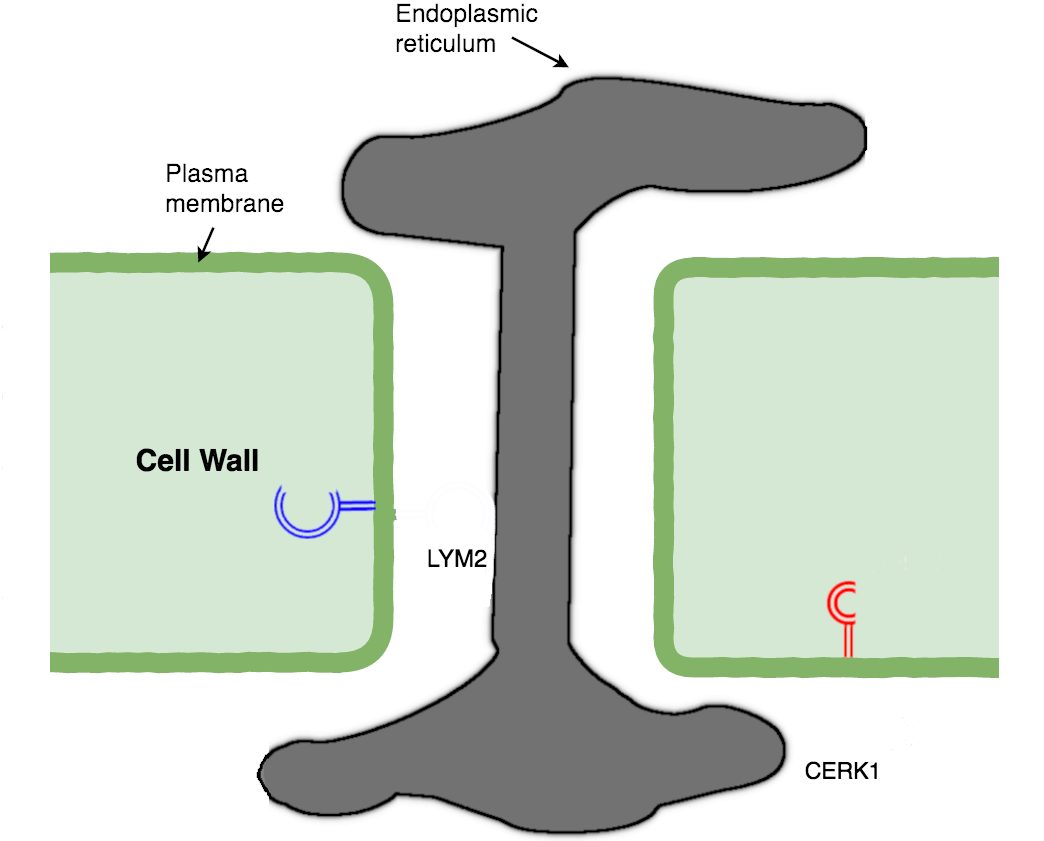
\includegraphics[width=0.5\columnwidth]{figures/original desmotubule.png}
  \caption[Plasmodesmata, \textit{lym2-1} and\textit{cerk2-1}diagram]{\label{fig:receptors}
    An illustrated plasmodesmata channel, with two
    known proteins involved in chitin signalling and plasmodesmata response. Red
    showing the canonical chitin detector CERK1, and in blue LYM2 a
    plasmodesmata localised protein}
\end{figure}

\section{Results}

\subsection{LYM2 is not required for a transcriptional response to chitin}

As LYM2, rather than CERK1 \cite{miyaCERK1LysMReceptor2007}, was previously
identified as being the essential protein for controlling symplastic
connectivity in response to chitin \cite{Faulkner2013} we hypothesised that it would also be vital
in regulating transcriptional responses to chitin. Therefore we used knock-out
mutants of LYM2 and CERK1 in the form of \textit{lym2-1} and \textit{cerk1-2}
respectively to ascertain what, if any, transcriptional differences occurred in
the absence of these receptor-like proteins.

With these mutants we applied either a chitin or water treatment, we then
performed RNA-seq on samples taken at 30 minutes and 6 hours post-application.
Initial analysis indicated that at both time-points, a significant
response to chitin is seen in both Col-0 and \textit{lym2-1} where several
hundred differentially expressed genes were found in both of these genotypes (figures:
\ref{subfloat:05hrDEGs} and \ref{subfloat:6hrDEGs})

In comparing the most differentially regulated genes we observe that very
similar profiles are shared by \textit{lym2-1} and Col-0, with minor differences
observed, through hierarchical clustering we show that at both time-points
\textit{lym2-1} and Col-0 are similar in the regulation of their most
differentially expressed genes (figure: \ref{fig:DEGS}). Thus the absence of
LYM2 does not impede a plants ability to activate a transcriptional response to chitin.


% Diff section ... 

\subsection{Temporal response to chitin is supported by LYM2}

To understand how a significant change to the transcriptome could occur in
\textit{lym2-1} whilst previous studies have shown lack of defence phenotype in
the same mutant, we compared temporal data of \textit{lym2-1} and Col-0 to find
an explanation.

When quantifying the number of DEGs between Col-0 and \textit{lym2-1} a much
higher level of mis-regulation is seen in \textit{lym2-1} at 30 minutes with
$\approx70\%$ more genes being differentially regulated than in wild-type (figure: \ref{subfloat:05hrDEGs}).
However, this effect is reversed with time, after 6 hours mis-regulation in
\textit{lym2-1} is seen to decrease by $\approx74\%$ whereas a reduction of $\approx52\%$ is
found in Col-0. This shift of regulation indicates that LYM2 impacts a plant's
ability to formulate a persistent defence response to chitin. 

\begin{figure}[!ht]
  \centering  
  \subfloat[Venn diagram of differential genes 30 minutes post-chitin
  treatment \label{subfloat:05hrDEGs}]{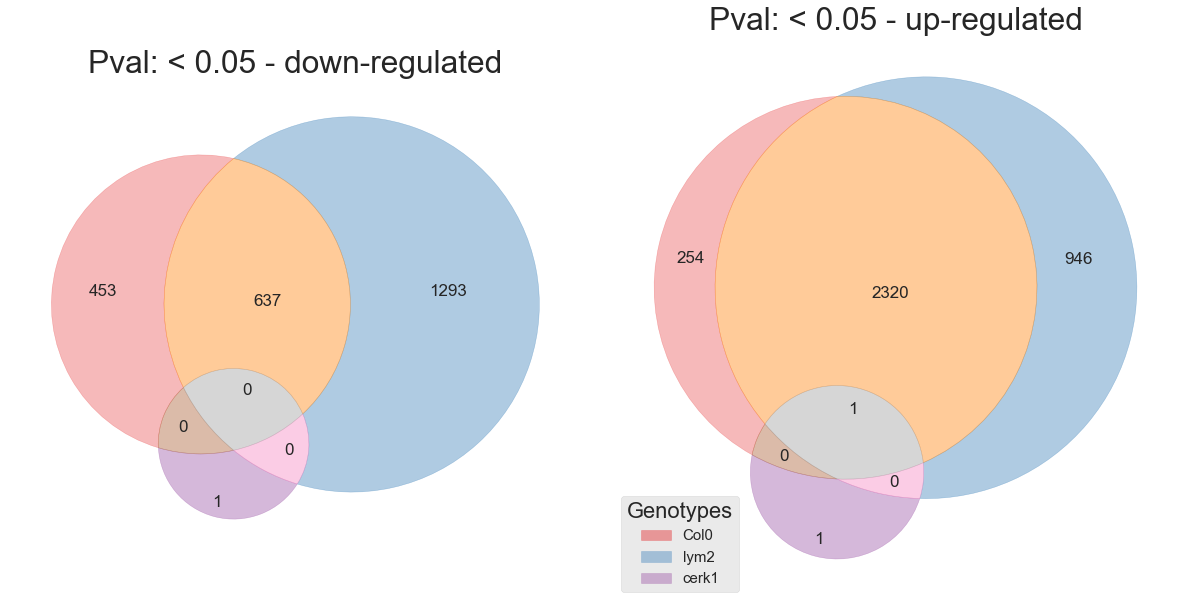
\includegraphics[width=0.9\columnwidth]{figures/vennTreatmentschitin.png}
  }
  \\
  \subfloat[Venn diagram of differential genes 6 hours post-chitin treatment \label{subfloat:6hrDEGs}] {%
    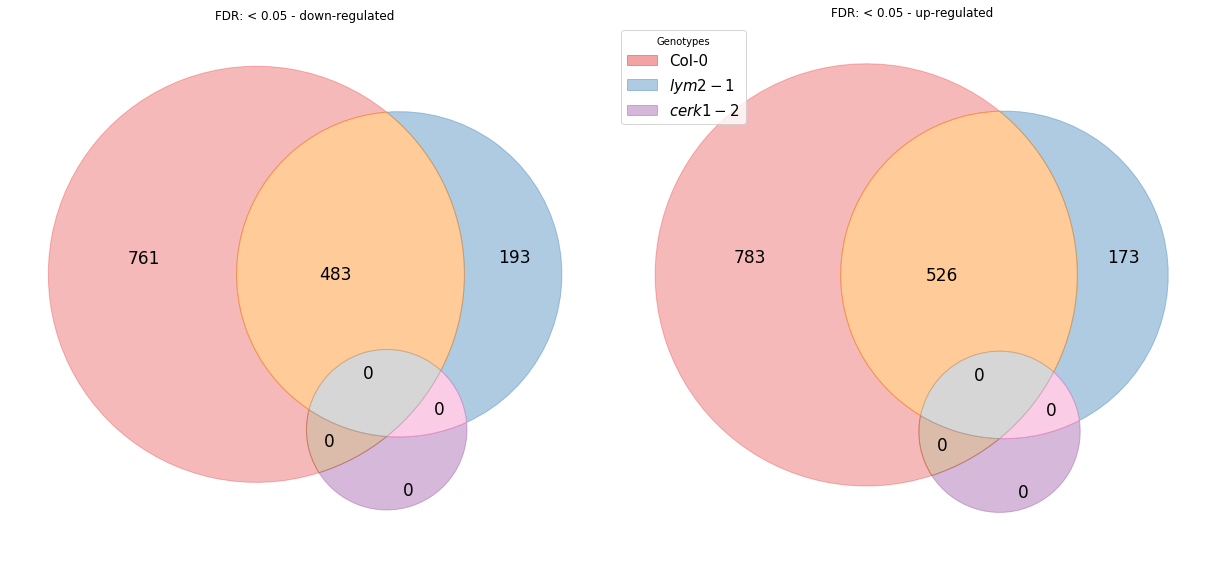
\includegraphics[width=0.9\columnwidth]{figures/vennTreatmentschitin6.png}}
  \caption[Number of differential genes found in chitin treated plants]{Shown
    left are genes down-regulated, right genes that are up-regulated in response
    to chitin. Colours give genotypes in study.}
  \label{fig:DEGsVenn}
\end{figure}

To further evaluate LYM2's temporal expression and to look for changes in degree
of gene expressions we looked at the number of genes with high-levels of
differential regulation for Col-0 and \textit{lym2-1} at both time-points. In doing this
analysis we note large reduction in genes with a high-value of LFC for both
genotypes but that \textit{lym2-1} gives the most drastic change in expression
profile (figure: \ref{fig:tmpHist})


\begin{figure}[!ht]
  \centering
  \subfloat[30 minutes post chitin application\label{subfig-1:tmpHist}]{%
    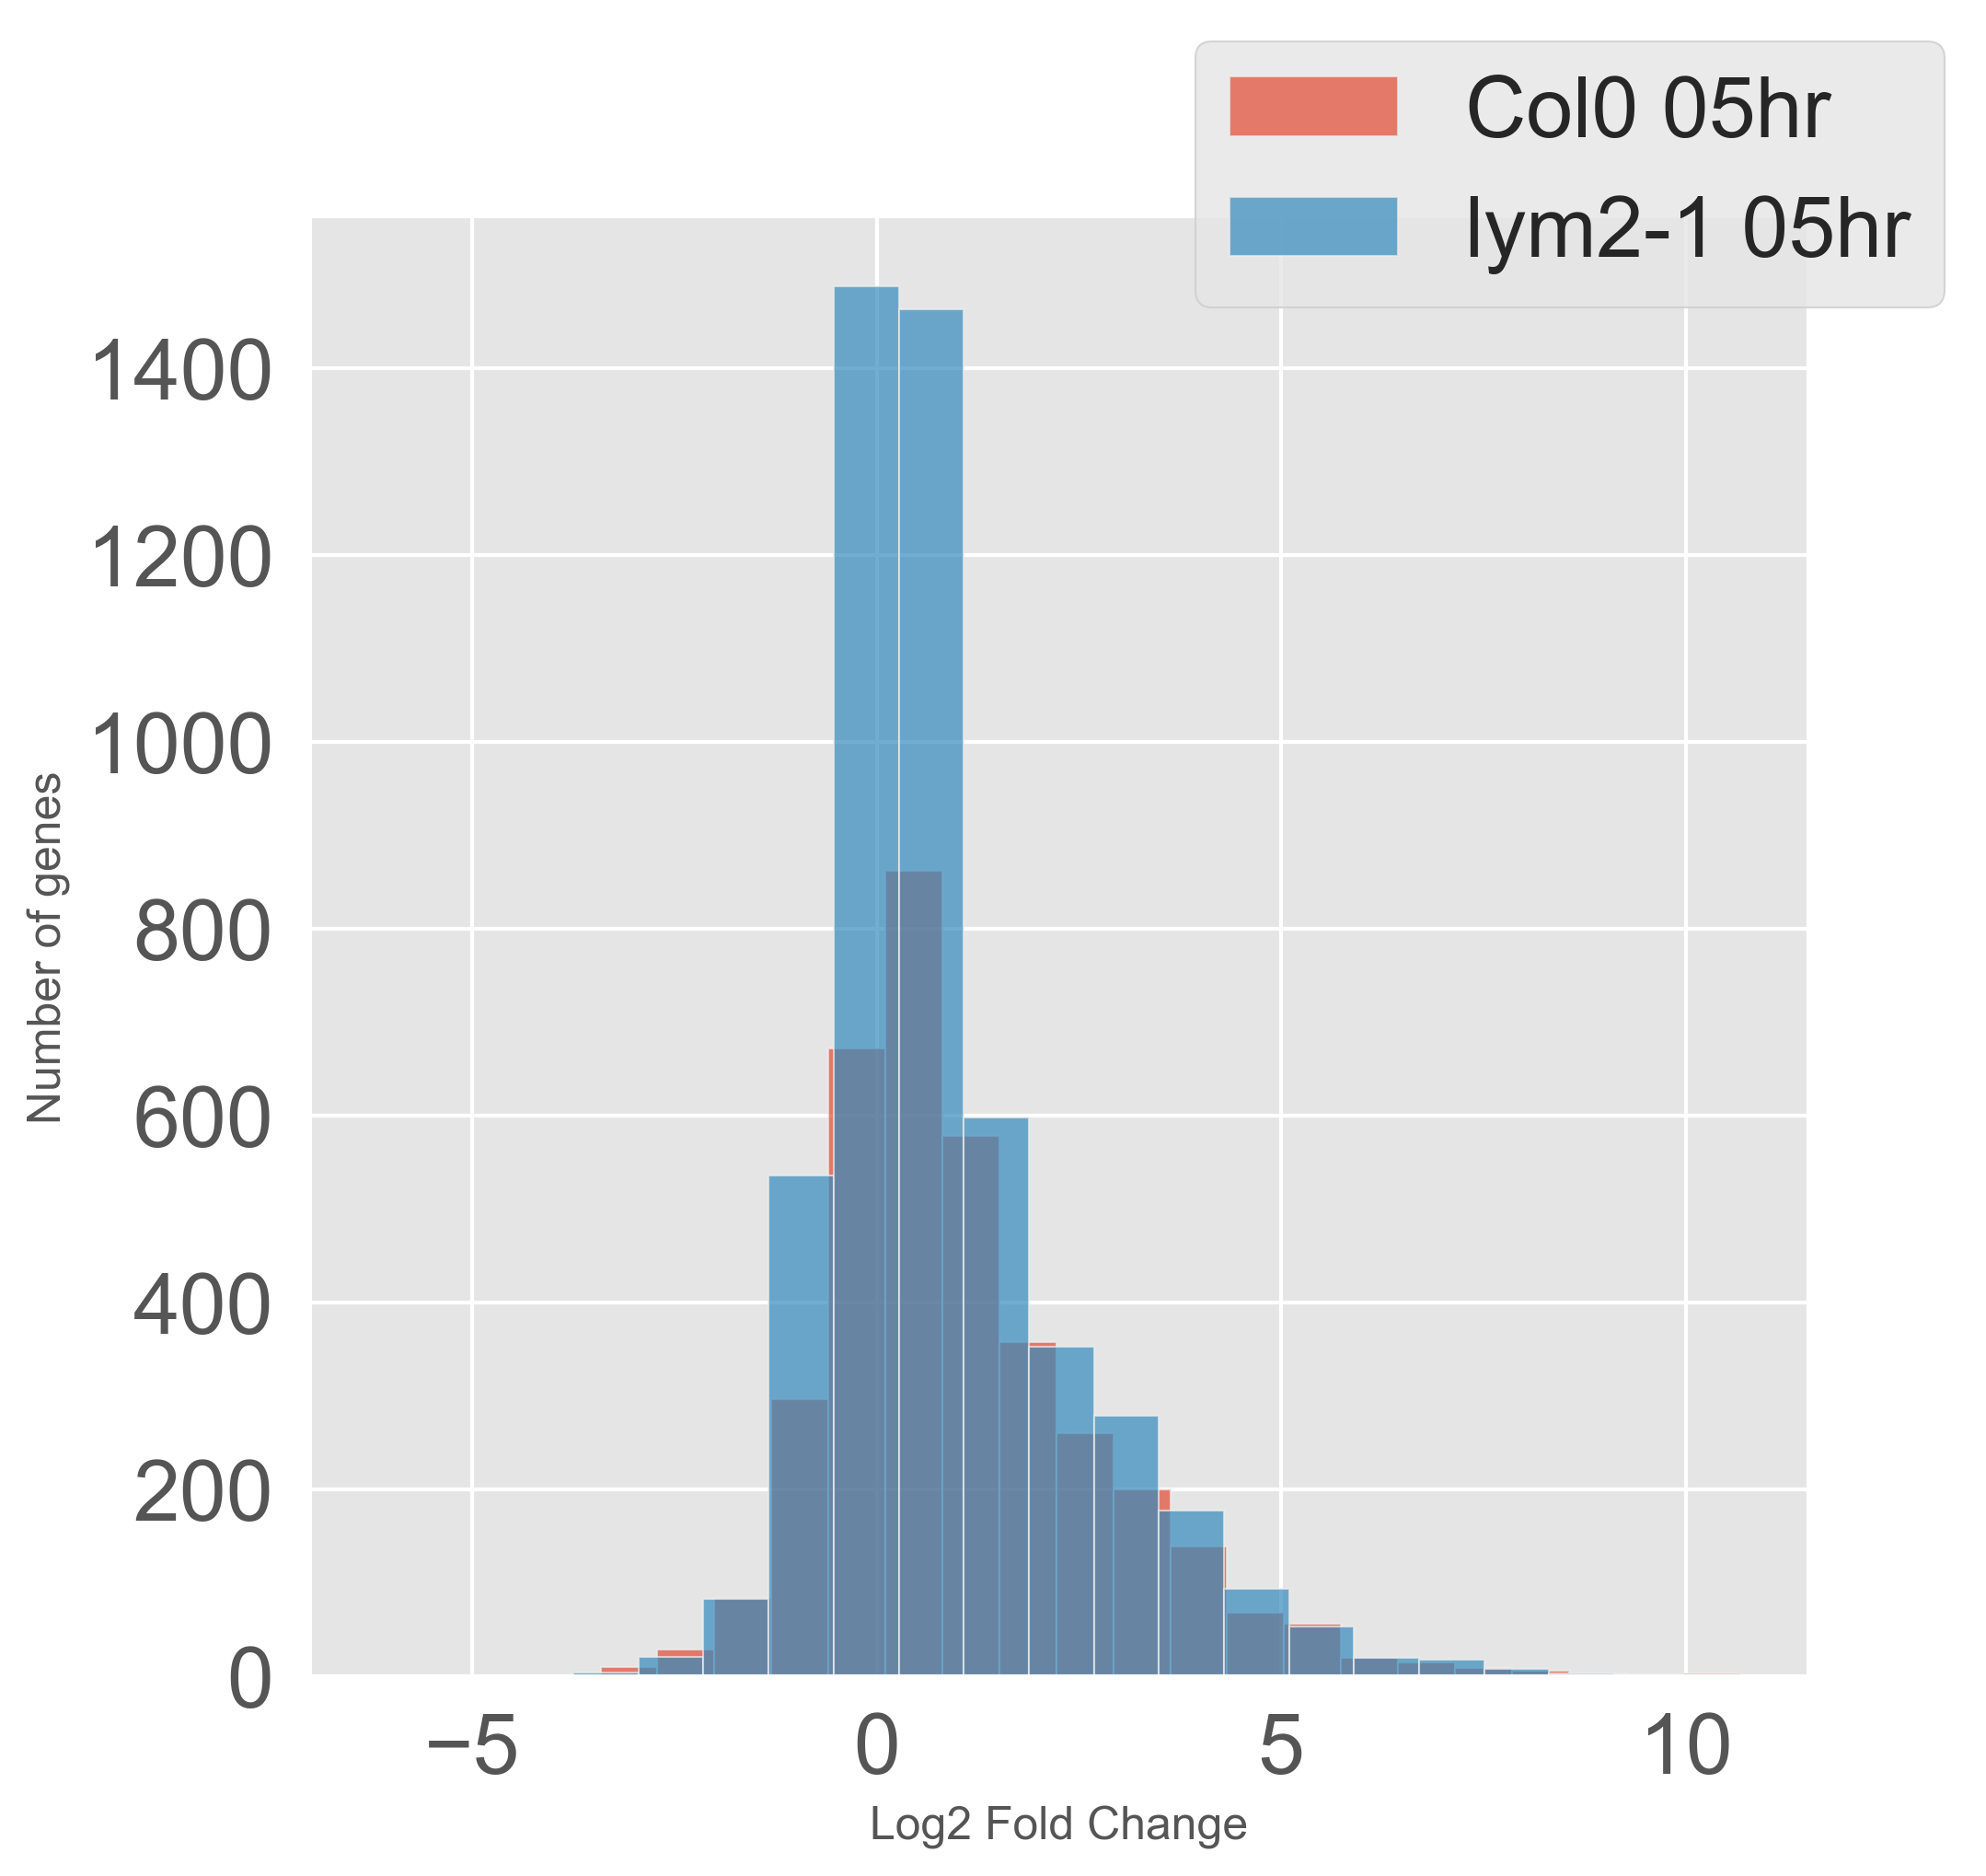
\includegraphics[width=0.4\columnwidth]{./figures/hist05hr.png}
  }
  \subfloat[6 hours post chitin application\label{subfig-2:tmpHist}]{%
    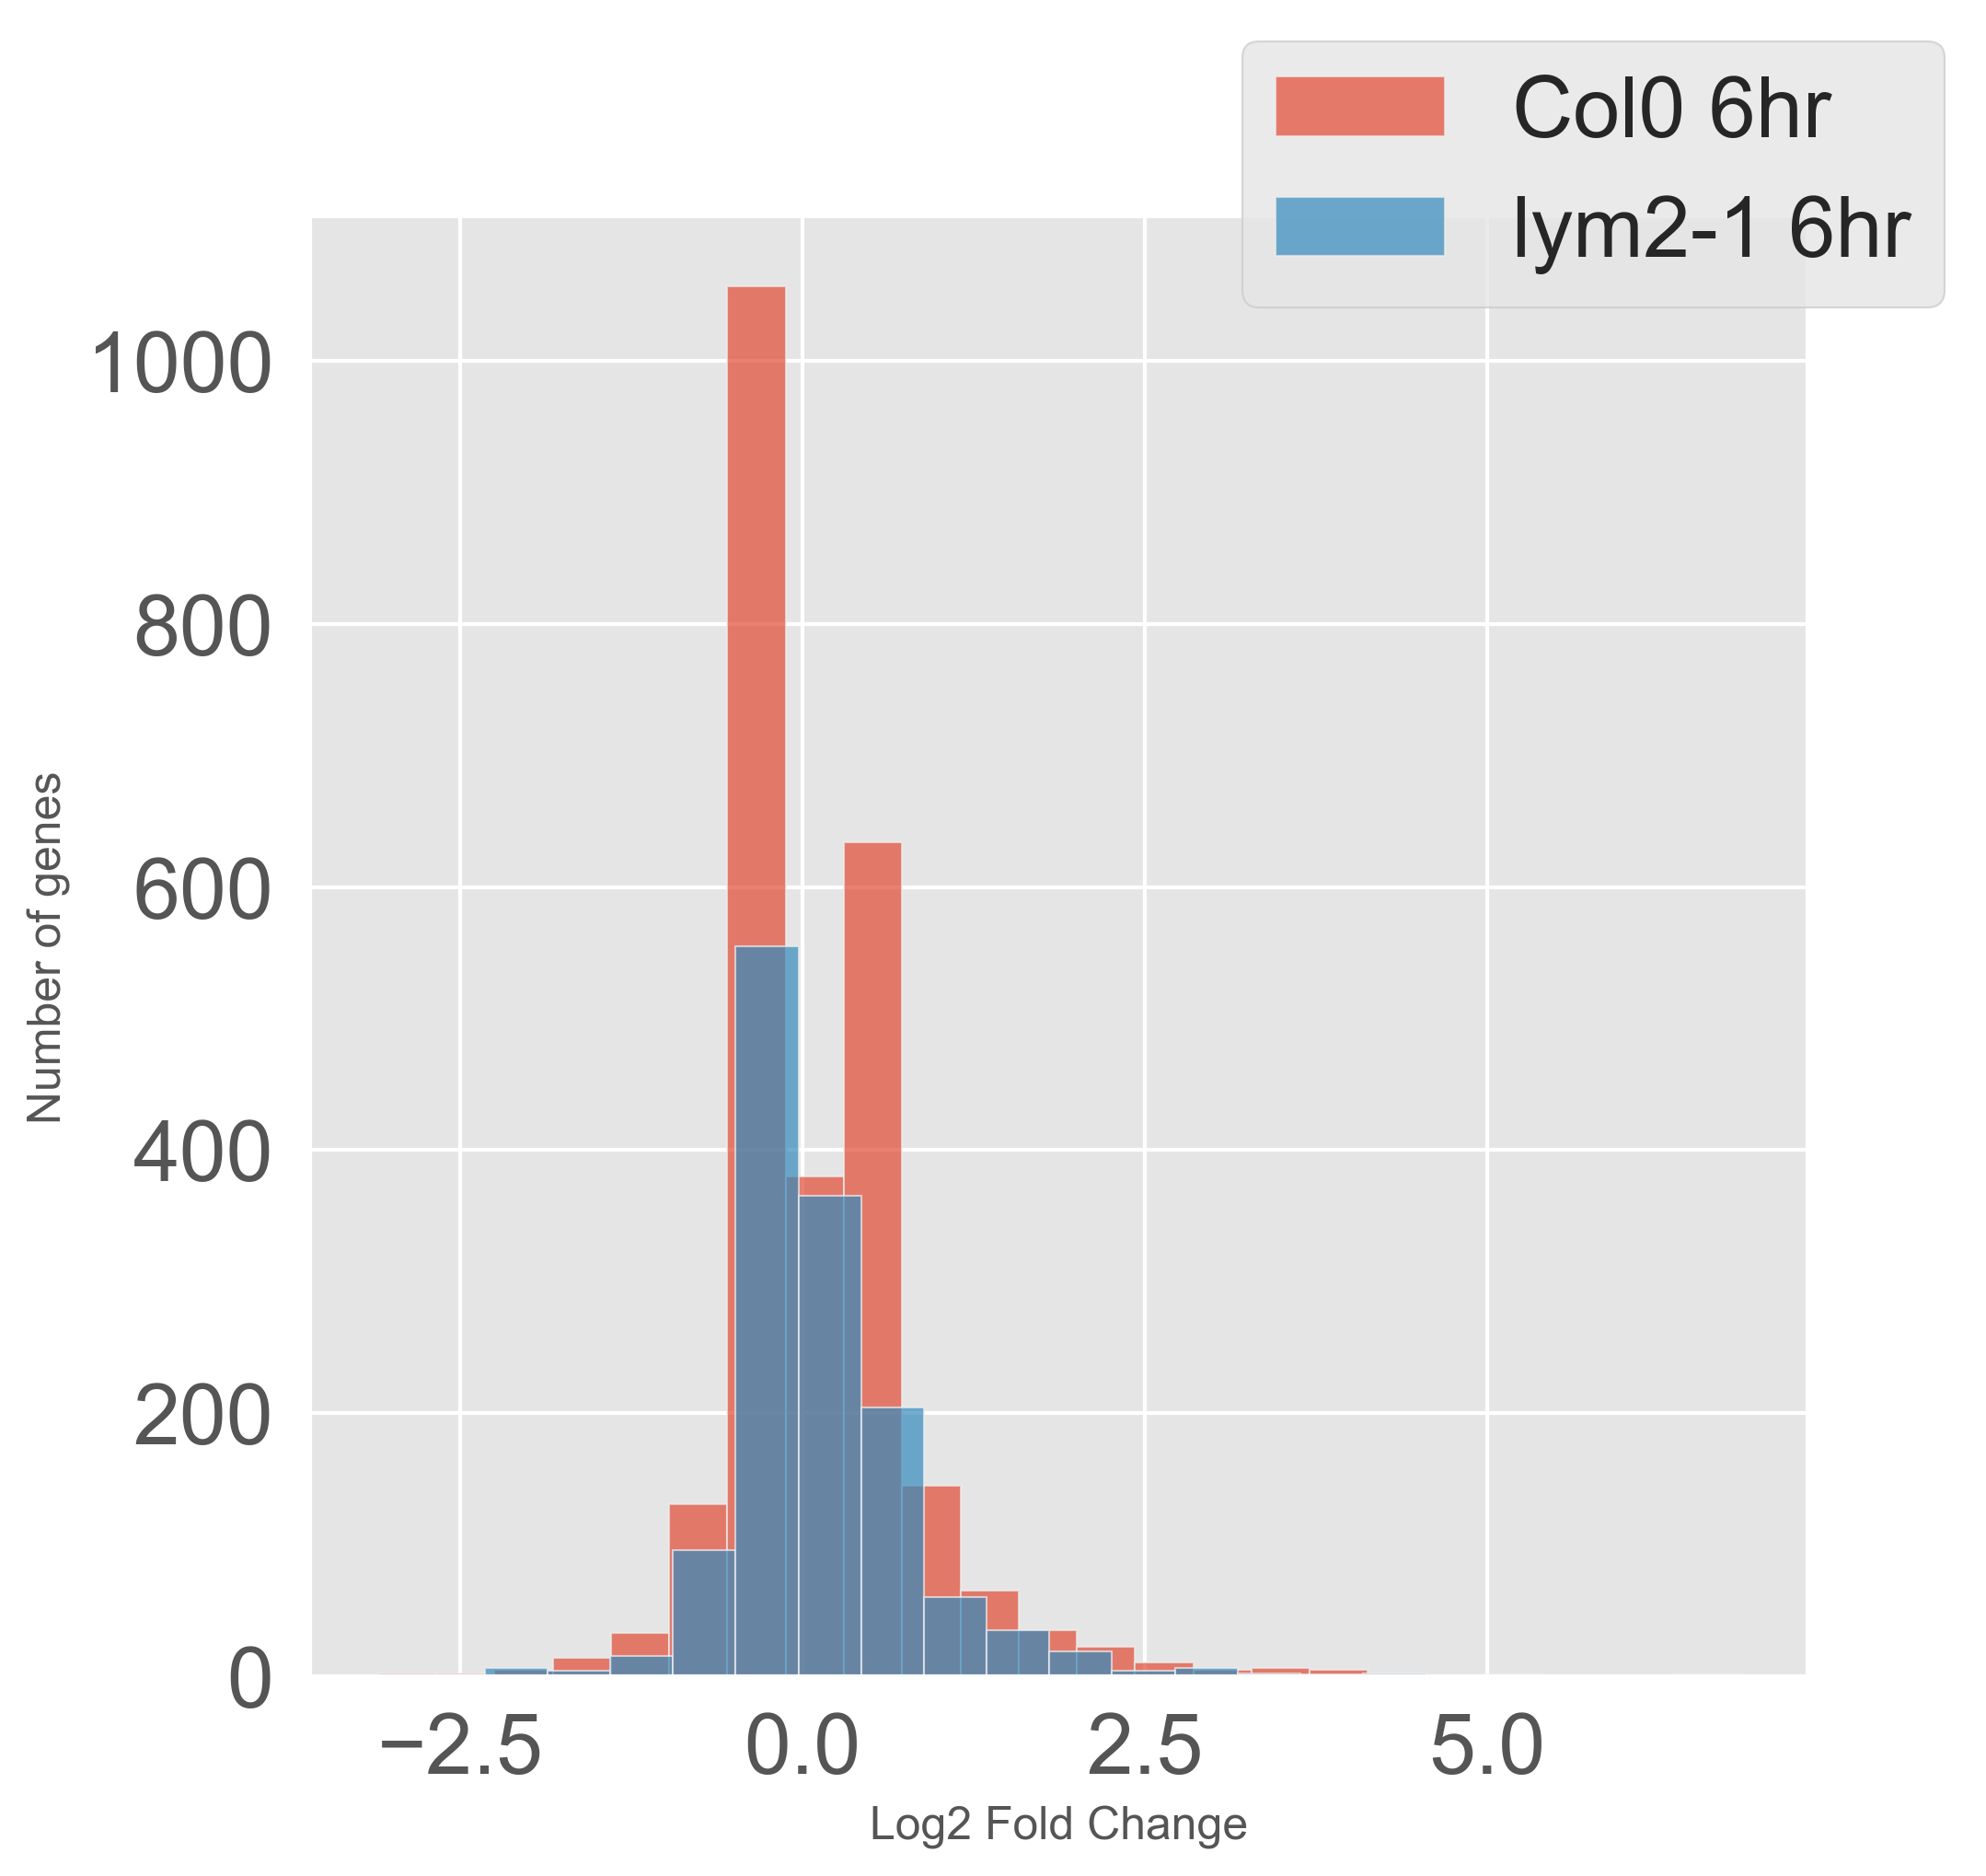
\includegraphics[width=0.4\columnwidth]{./figures/hist_6hr.png}
  }
  \caption[Temporal histograms of RNAseq data]{Temporal histograms. In red Col-0 DEGs are shown, \textit{lym2-1} in
    blue. Positive values show up-regulation and negative down in response to
    chitin treatments}
  \label{fig:tmpHist}
\end{figure}


\subsection{CERK1 is not required for chitin perception}

CERK1 has been canonically described as an essential protein in chitin
perception \cite{miyaCERK1LysMReceptor2007,
  shinyaFunctionalCharacterizationCEBiP2012} and its relationship with
symplastic defence has been a point of interest since it was shown to not be
required for plasmodesmatal closure in response to chitin. It would therefore be
reasonable conjecture to expect that \textit{cerk1-2} produces no DEGs between a
chitin or a water treatment. 

Surprisingly, in our experiments \textit{cerk2-1} produced 3 DEGs after 30
minutes, whereas Col-0 and \textit{lym2-1} show to have 3664 and 5196
respectively (figure: \ref{subfloat:05hrDEGs}). Whilst the effect seen in
\textit{cerk1-2} is greatly subdued, our data indicates that CERK1 is essential
in enabling many processes but, some transcriptional response to chitin is still
possible. Furthermore, as our 6 hour post-treatment data revealed no differences
in \textit{cerk1-2} we propose that CERK1 is not required for chitin perception
and that another unknown protein is able to perceive exogenous chitin and enable
plasmodesmata closure. 

% With this our data also maintains and strengthens the established
% conjecture that CERK1 and LYM2 are independent chitin response signalling pathways
% \cite{Faulkner2013, miyaCERK1LysMReceptor2007,
%   narusakaPresenceLYM2Dependent2013}.

\begin{figure}[!ht]
  \centering
  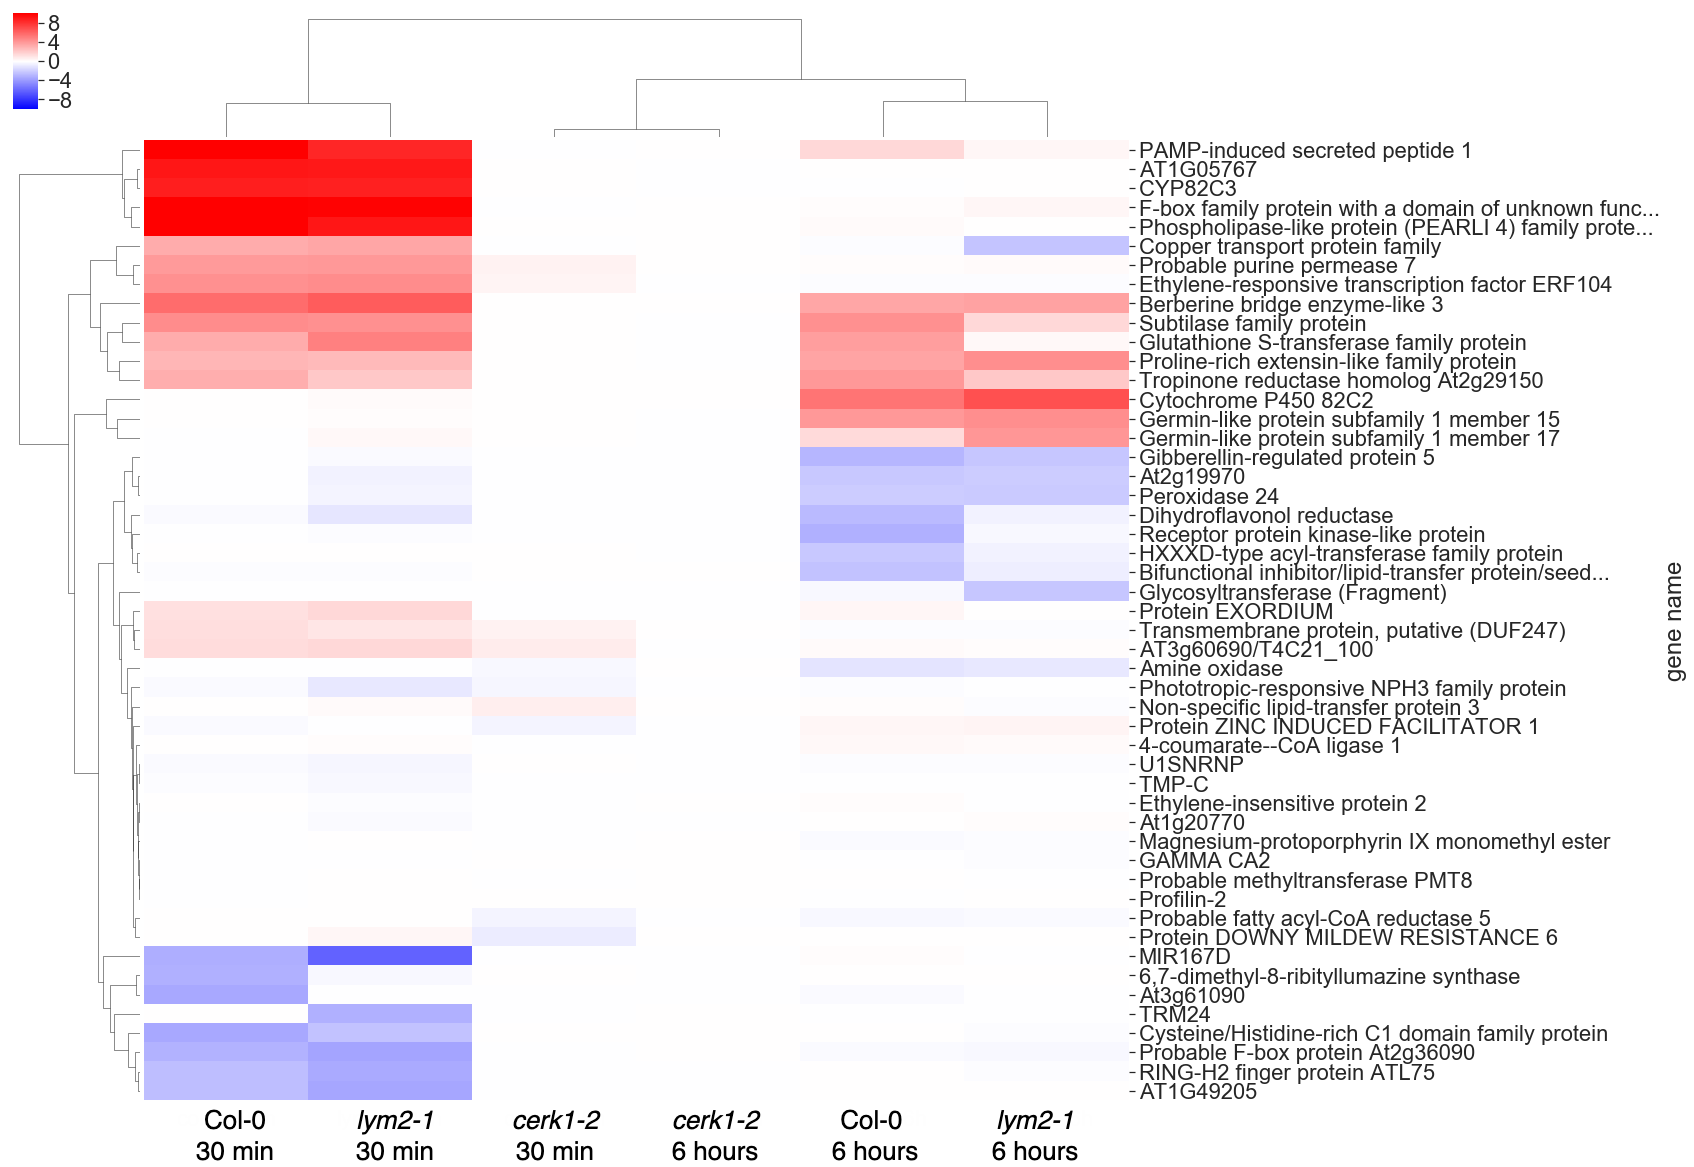
\includegraphics[width=\columnwidth]{figures/allDEGs.png}
  \caption[Most differentially regulated  genes in response to
  chitin]{\label{fig:DEGS} Most differentially regulated  genes in response to
    chitin. 10 genes from each sample were selected, 5 most up-regulated and 5
    most down-regulated. Values were then found selected from all samples for
    comparison. Colour indicates log2 fold change. Columns represent different
    genotype's at different time-points. Hierarchical clustering is used column
    and row wise to group similarly patterned values}
\end{figure}


\subsection{Down-regulation of DMR6 causes plasmodesmata closure}

With the unexpected discovery of differential genes in \textit{cerk1-2}'s
response to chitin, we investigated the profile of these genes to verify their
differences across genotypes and to check basal differences in response to
water. We did this by comparing normalised count data for transcripts of the three
differential \textit{cerk1-2} genes and reviewing their function in order to
gain insight to how they are active in spite of CERK1's absence.

The sole down-regulated gene exclusively found in \textit{cerk1-2}, AT5G24530
(DMR6) has previously been described as enhancing susceptibility to downy mildew
\cite{DOWNYMILDEWRESISTANT}, these data could suggest that a secondary fallback
mechanism is activated only when CERK1 is not present (figure:
\ref{subfig-1:cerk}).

Two other genes that appear to be differentially regulated in \textit{cerk2-1}
AT5G59320 (LTP3) and AT3G60690 (SAUR59) may be worth further consideration. LTP3
has been shown to be involved with abscisic acid, an important signalling
molecule in abiotic/biotic stress \cite{vishwakarmaAbscisicAcidSignaling2017} and
SAUR59 is indicated to be a highly mobile transcript
\cite{thiemeEndogenousArabidopsisMessenger2015} and thus potentially involved in
cell-cell communication of stress (Figures \ref{subfig-2:cerk} and
\ref{subfig-3:cerk}). Though, given that similar trends are seen in
\textit{lym2-1} and Col-0 in terms of regulation-direction compared to water
treatments their interest is devalued.

Given the nature of DMR6, its behaviour in both Col-0 and \textit{lym2-1}, our
current data would allow for the hypothesis that DMR6 is able to trigger
plasmodesmata closure, independently from other methods available to Col-0.

%  This indicates that chitin perception is not wholly dependant
% on CERK1, as previously thought.  


\begin{figure}[!ht]
  \subfloat[AT5G24530 (DMR6), the single gene found in \textit{cerk1-2} mutants
  which shows a down-regulation in response to chitin \label{subfig-1:cerk}]{%
    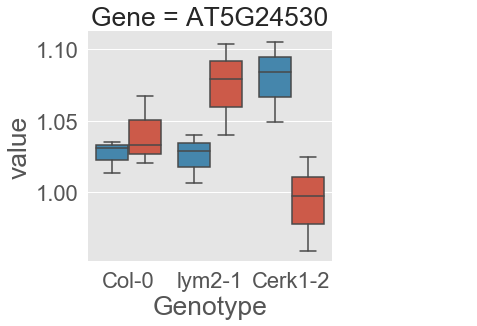
\includegraphics[width=0.45\columnwidth]{./figures/cerk_genes_AT5G24530.png}
  }
  \qquad 
  \subfloat[AT5G59320 (LTP3), Significantly up-regulated in \textit{cerk1-2}
  but not in Col-0 or \textit{lym2-1} \label{subfig-2:cerk}]{%
    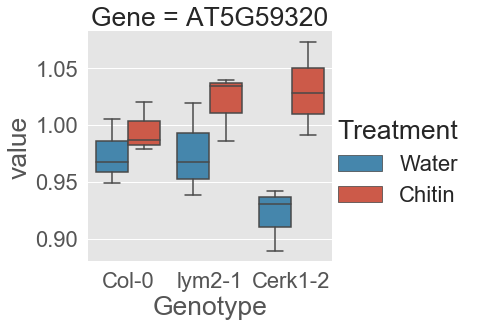
\includegraphics[width=0.45\columnwidth]{./figures/cerk_genes_AT5G59320.png}
  }\\
  \subfloat[AT3G60690 (SAUR59), Significantly up-regulated in response to
  chitin for all genotypes in study \label{subfig-3:cerk}]{%
    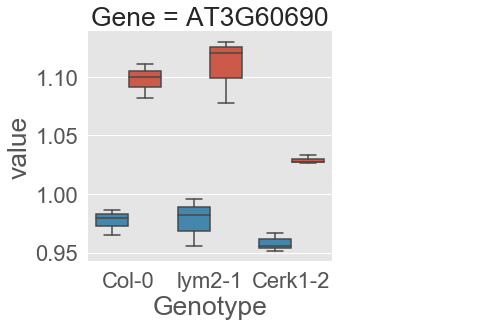
\includegraphics[width=0.45\columnwidth]{./figures/cerk_genes_AT3G60690.png}
  }
  
  \caption[Differential \textit{cerk1-2} genes at 30 minutes post-chitin treatment]{Genes which were found to have a differential regulation in the
    \textit{cerk1-2} genotype. Presented for comparison are the values in both
    Col-0 and \textit{lym2-1}, Y values are given as normalised transcript counts
    for each transcript across different treatments (Normalisation was performed
    gene-wise, values are comparative across treatments but not between genes).
    Blue colour in boxplots represents water treatments, red as chitin }
  \label{fig:cerk}
\end{figure}




\subsection{LYM2 has a highly specific role in defence regulation}

To better ascertain what effect the transcriptional changes observed in
\textit{lym2-1} were having, if they were not leading to plasmodesmatal closure we
performed Gene ontology (GO) term analysis on the DEGs found. Whilst having
hundreds of differential genes both Col-0 and \textit{lym2-1} have a lot of
similarities. Firstly, they show very few GO-terms being enriched/purified.
Secondly they show a great deal of overlap of those that have been found
(figure: \ref{fig:05hrGO}).

This analysis indicates that a large part of the transcriptomic disruption
caused by chitin results in seemingly disconnected processes (thus the low
number of significant GO terms to number of DEGs). The terms which do create interest are
``response to chitin'' which indicates that Col-0 has a sub-set of DEGs that are
down-regulated exclusively (figure \ref{fig:05hrGO}), and ``defense response to bacterium''
which conversely shows an exclusive set of \textit{lym2-1} genes that are
down-regulated in response to chitin (supplemental
tables \ref{cha:suppltbl}).

However, closer inspection of data reveals that expression profiles of these groups
are similar and that repeated experiments could give contradictory results
(supplemental figures \ref{fig:respchitin} and \ref{fig:defbacterium}).


\begin{figure}[ht]
  \centering
  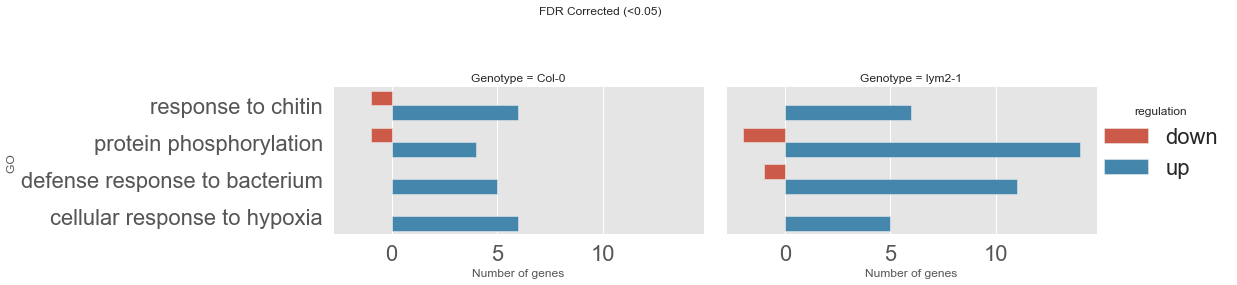
\includegraphics[width=\columnwidth]{figures/05hrGO.png}
  \caption[GO terms found in Col-0 and \textit{lym2-1} at 30
    minutes post chitin treatment]{\label{fig:05hrGO} GO terms found in Col-0 and \textit{lym2-1} at 30
    minutes post chitin treatment. Up-regulated terms are given as blue and down
  in red. Down-regulated terms are shown as negative values to indicate that the
  respective term has genes which are down-regulated}
\end{figure}


\subsection{Analysis of temporally different genes}

As \textit{lym2-1} displayed a sharp decline in number of DEGs over time, whilst Col-0 had
a more gentle response we sought to find genes at 30 minutes
post-treatment that may control down-stream expression. To do this we devised a
method of selecting genes based on opposing temporal expression. We firstly gave
all DEGs a two point coordinate, one for LFC at each time-point, then reduced
our genes of interest to those with opposing directions. This gave genes which
were either up-regulated at 30 minutes and down-regulated at 6 hours or the
reverse (figure: \ref{fig:diverg}).


\begin{figure}[!ht]
  \centering
  \subfloat[Genes found when selecting for FDR < 0.05 \label{subfig-1:diverg}]{%
    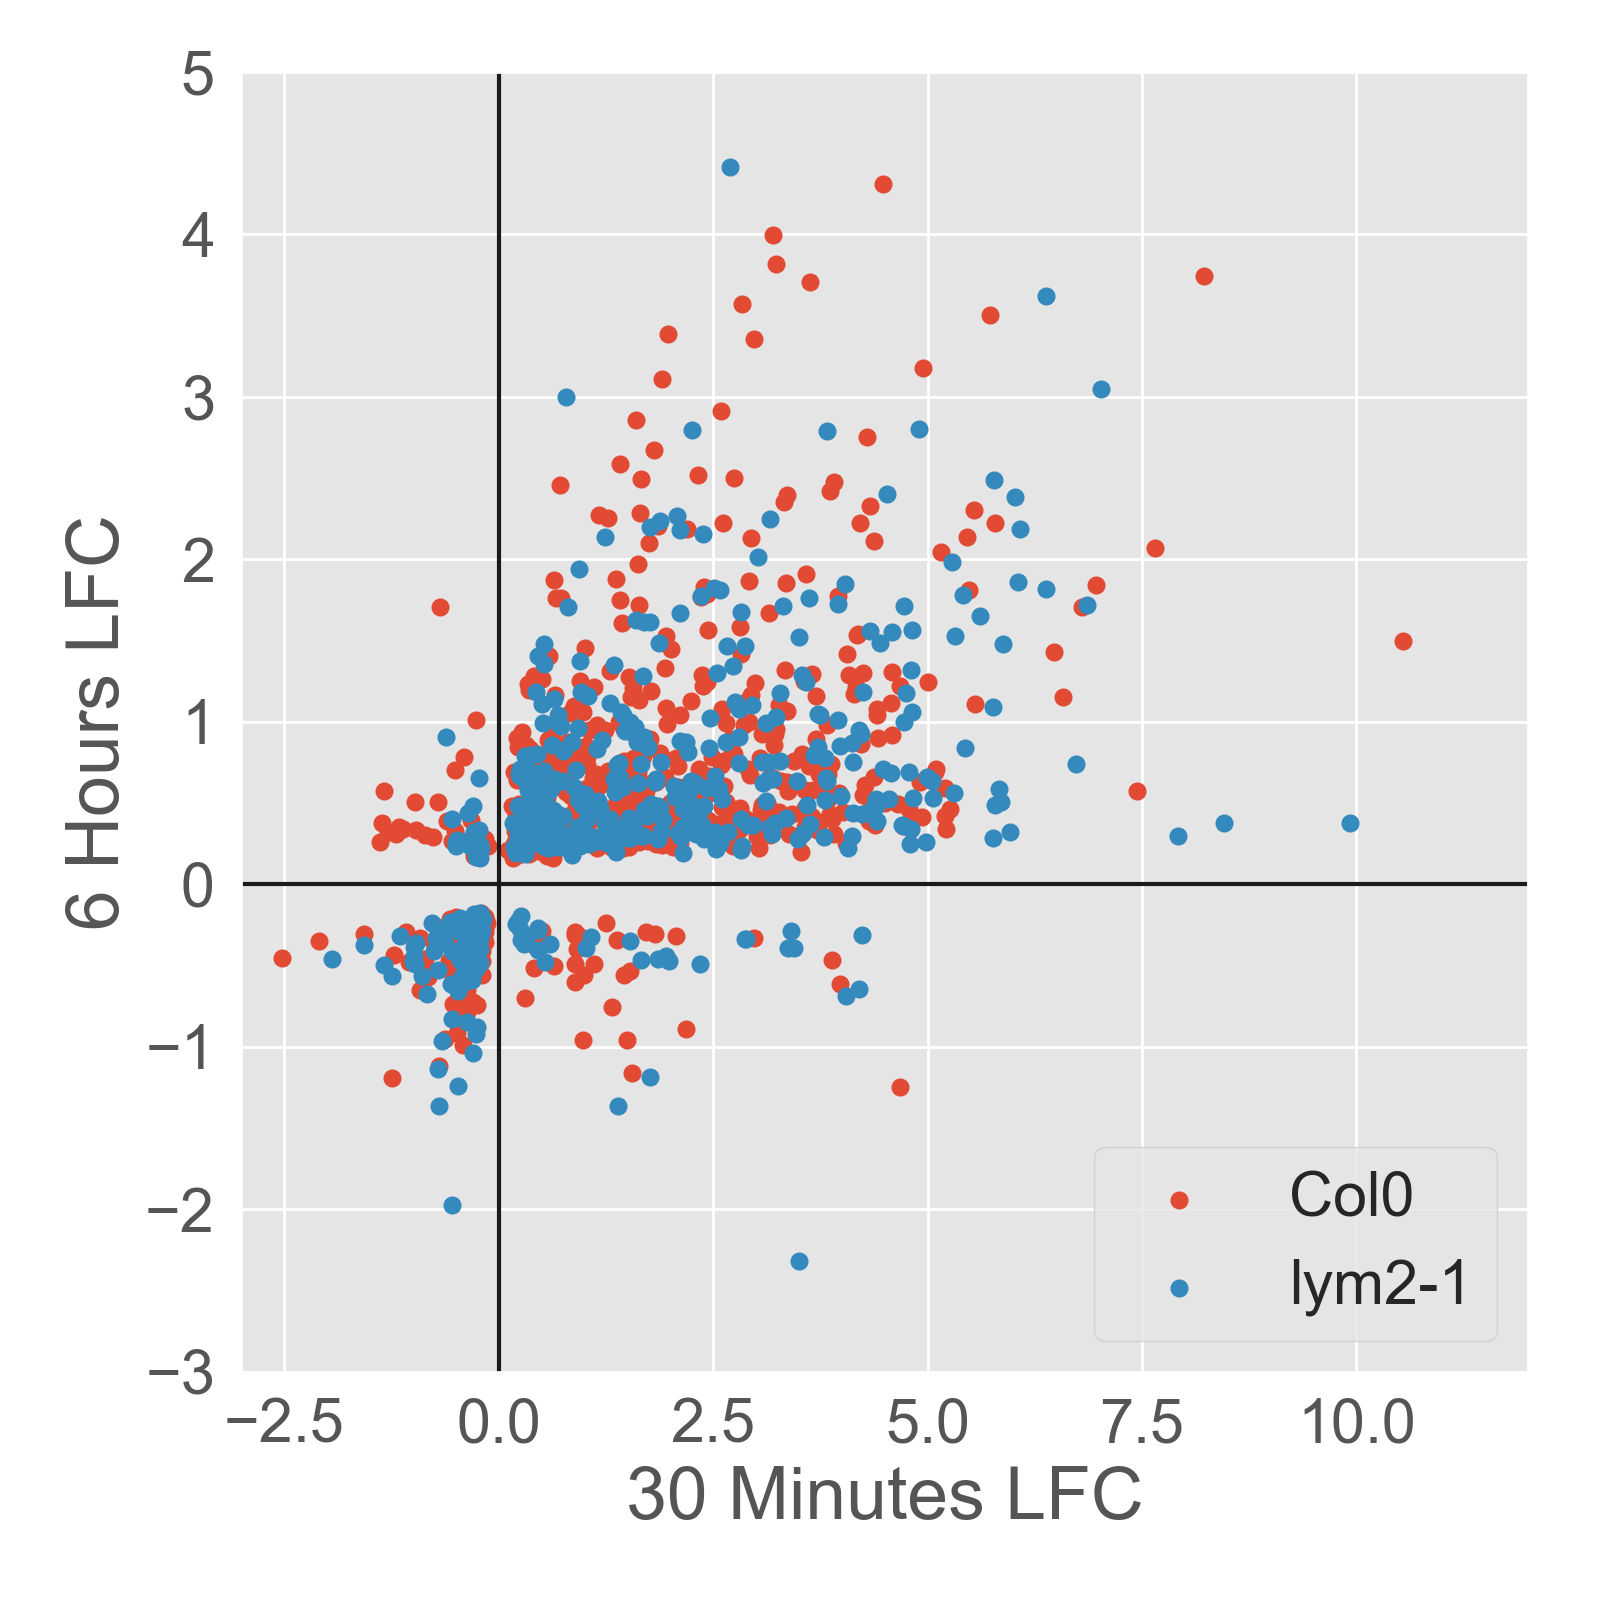
\includegraphics[width=0.5\columnwidth]{./figures/divergingGenes_all.png}
  }
  \subfloat[Genes found when selecting for opposite expression patterns\label{subfig-2:diverg}]{%
    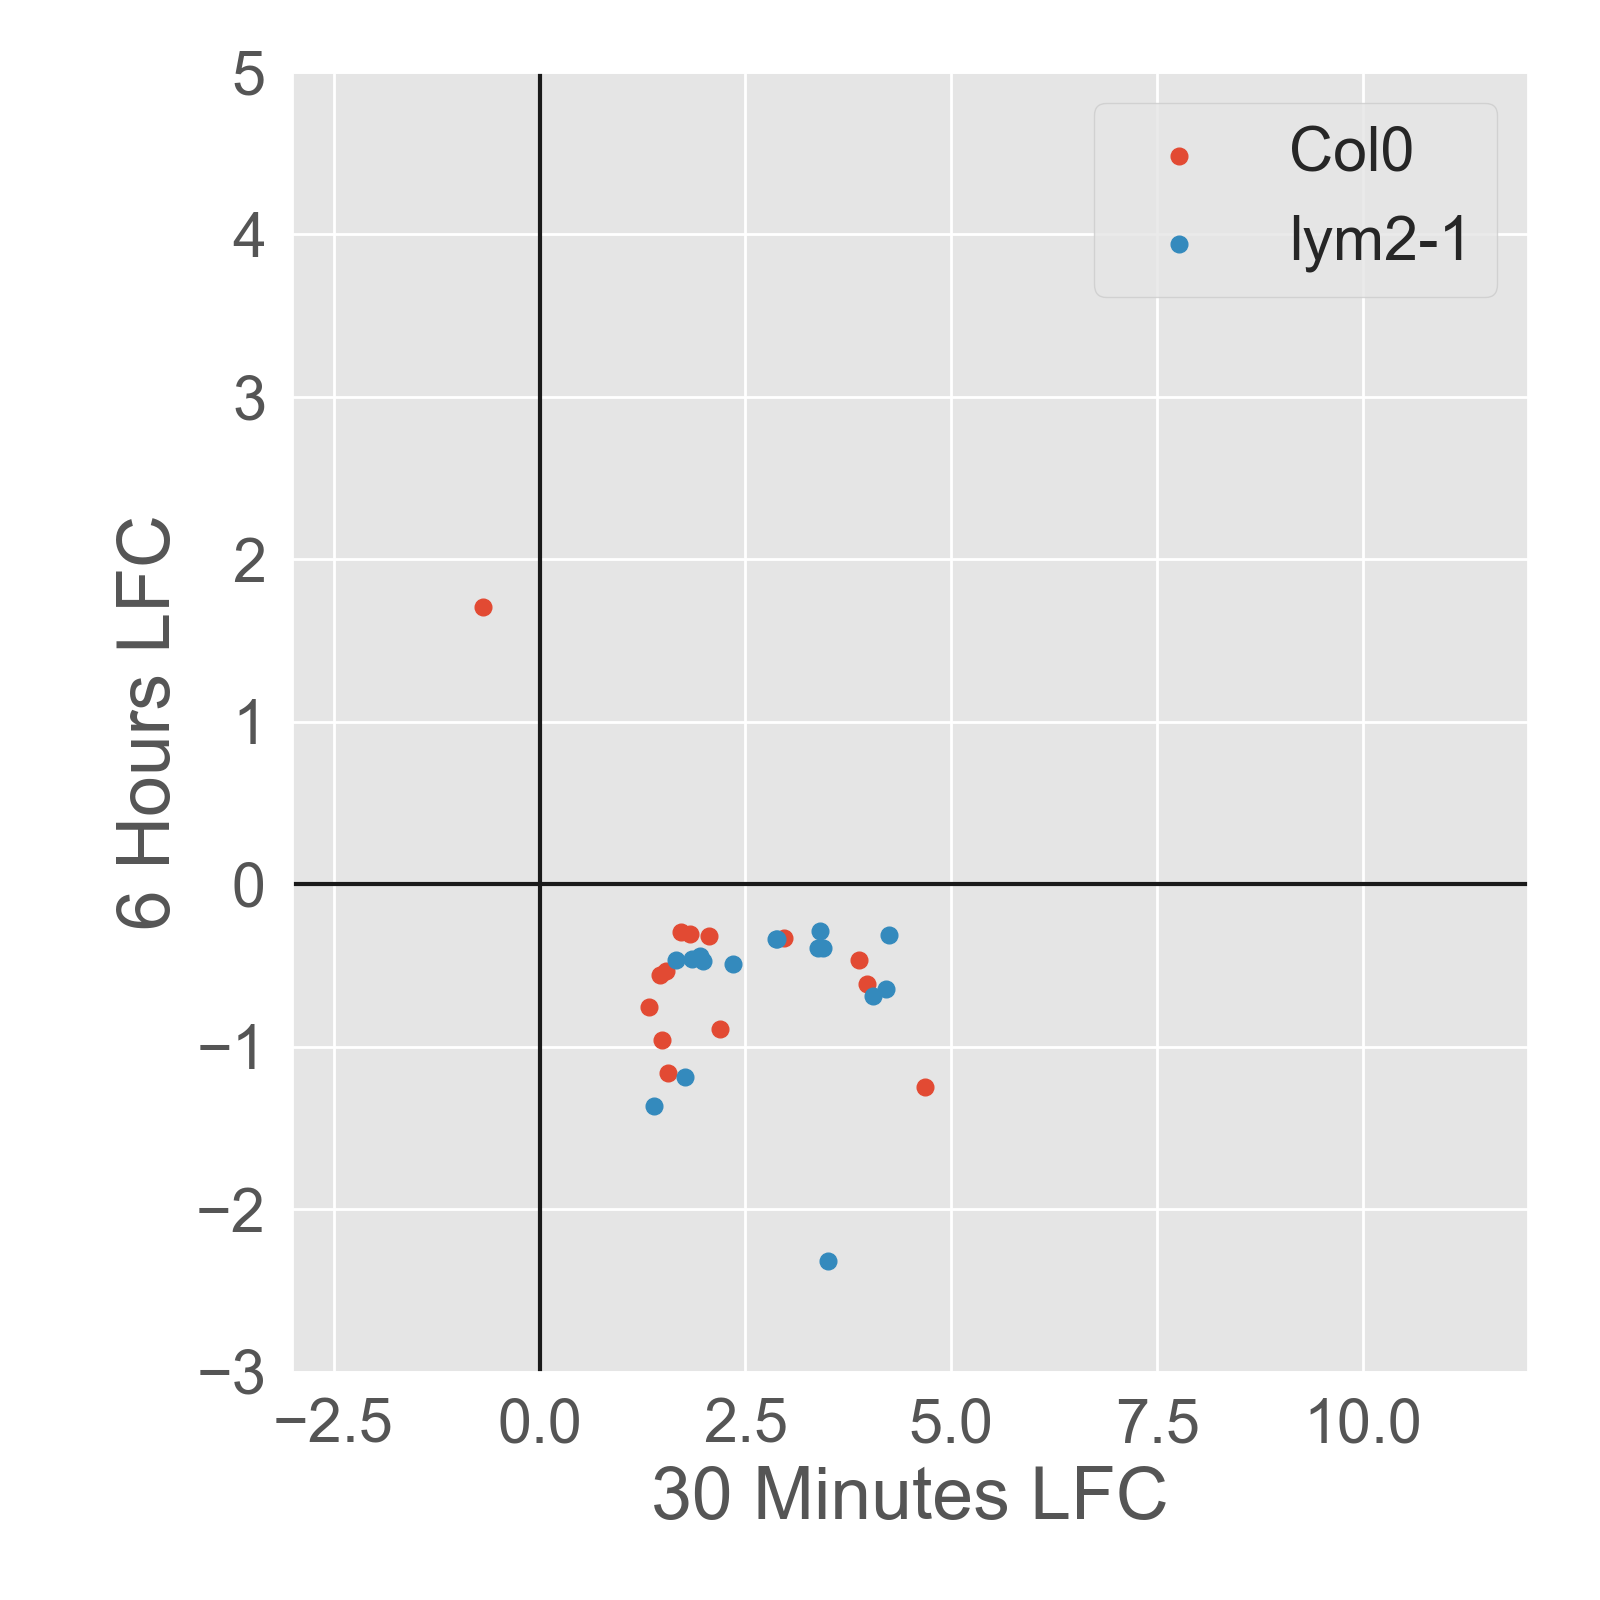
\includegraphics[width=0.5\columnwidth]{./figures/divergingGenes.png}
  }
  \caption[Differential genes plotted by expression at two time points]{DEGs plotted by time after chitin application. X axis gives
    expression at 30 minutes, Y 6 hours. Colour shows genotype, Col-0 is shown
    in red and \textit{lym2-1} in blue}
  \label{fig:diverg}
\end{figure}

From this refined selection process we investigated one gene for each group, we
selected the gene with the largest LFC difference between time-points. Upon
comparison we found very little difference between Col-0 and \textit{lym2-1}
expressions, though we note that a certain level of basal differences (those
seen in water treatment controls) may explain some of these lack of differences
(figure: \ref{fig:interestinggenes}).

\begin{figure}[!ht]
  \centering
  \subfloat[AT3G04070 (NAC DOMAIN CONTAINING PROTEIN 47)\label{subfig-2:interest}]{%
    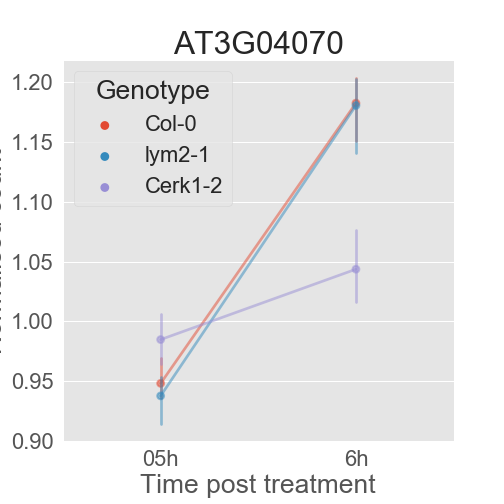
\includegraphics[width=0.7\columnwidth]{./figures/interestingGenes_AT3G04070.png}
  }\\
  \subfloat[AT5G52710 (Copper transport associated gene) \label{subfig-1:interest}]{%
    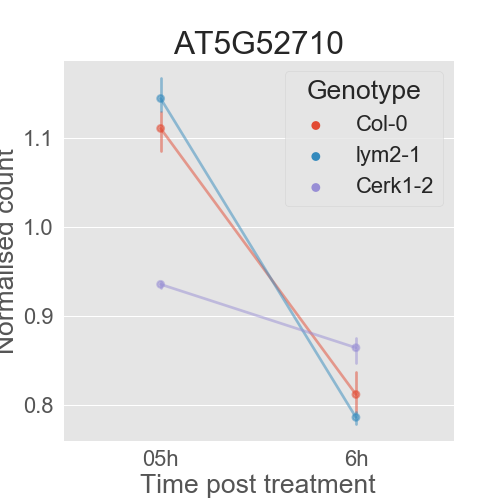
\includegraphics[width=0.7\columnwidth]{./figures/interestingGenes_AT5G52710.png}
  }
  \caption[Genes which have conflicting directions of regulation across time]{Genes which have conflicting directions of regulation across time.
    Coloured lines represent genotype, time-point on X axis, normalised
    expression count given on Y. Left plot shows expression of water control
    plants, right plot after chitin application}
  \label{fig:interestinggenes}
\end{figure}


\section{Discussion}

The importance of plasmodesmata in both initial localised responses to pathogens
\cite{chevalChitinPerceptionPlasmodesmata2019} and in later whole-plant
responses (systemic acquired resistance (SAR))
\cite{chevalPlasmodesmalRegulationPlant2018} cannot be understated. It is
therefore crucial that we understand and dissect the processes that lead to
these responses. In this study we have been able to elude to behavioural
dynamics of two key proteins in chitin defence. We have confirmed that, as
previously thought, CERK1 is not required for chitin perception and that it is
also not required for a transcriptional response. From this understanding we can
suggest that Protein DOWNY MILDEW RESISTANCE 6 (DMR6) has an important role in
the reduction of symplastic connectivity when CERK1 is absent.

From the behaviour of DMR6 we further give evidence that both LYM2 and CERK1 are
not necessary for a transcriptional response to chitin, albeit minimal. This
suffices to suggest that at least one other protein is capable of perceiving
chitin in some form.

With such an interesting change observed in the \textit{lym2-1} genotype, a more
refined time-course could uncover the exact point of change, as well as what
particular genes (or lack of) lead to the decline in transcriptomic activity

To consolidate these data with their role in symplastic defence a
spatial-temporal phenotypic data set on plasmodesmata state during infection
would be required. Many questions on these data could be resolved if the
behaviour of plasmodesmata could be correlated with the DEGs given here. 



\section{Materials and methods}

\subsection{Plant materials}
An RNA-seq assay was performed on three genotypes of Arabidopsis Thaliana to
test for transcripts unique to chitin perception. Col-0 used as a control,
as well as \textit{lym2-1} and \textit{cerk2-1} which are knock-out mutants of
their respective chitin perception proteins. 

All three of these genotypes were grown on plates for 7 days before transferred
to liquid media for 7 days. Samples were treated on day 14. Either a chitin or
water treatment was added and mixed into sample suspension. Samples were taken
at 30 minutes post treatment and at 6 hours. Whole seedlings were taken, pooled
in groups of 10 and sequenced together for robustness. Three replicates of each
genotype, treatment and time point were produced (36 samples in total).


\subsection{Computational methods}

Data were pre-processed firstly through removing adaptor sequences, with
\textit{trimmomatic} \cite{bolgerTrimmomaticFlexibleTrimmer2014}. Sanity checks
were performed using \textit{fastqc} \cite{andrewsBabrahamBioinformaticsFastQC}.
Alignment was carried out using a combination of \textit{samtools} and
\textit{hisat2} \cite{liSequenceAlignmentMap2009}. Finally, \textit{htseq-count}
was used to prepare sequence counts from trimmed and aligned RNA-seq data
\cite{kimHISATFastSpliced2015}. Preparation of count data used the method
described by \citet{loveModeratedEstimationFold2014a} and normalised transcript
counts were created using \textit{DESEQ2}
\cite{piperCountNormalizationDESeq22017}.

With these normalised data, we calculated the false discovery rate (FDR) value
for chitin compared to water treatments of each genotype at each time point. We
specified that all genes with an FDR$< 0.05$ would be considered significant.
For further down-stream gene-ontology (GO) analysis we used
\cite{klopfensteinGOATOOLSPythonLibrary2018}, and further limited genes of
interest to having a Log2 Fold Change (LFC) of $>2$ to select only genes with a
high degree of difference from their water treatment.



\end{document}


%%% Local Variables:
%%% mode: latex
%%% TeX-master: "../main"
%%% End:
